\chapter{Selectie protocollen}
\label{selectie}

Om het onderzoek binnen de beschikbare tijd te houden is er in overleg met de Blockchain Expert voor gekozen om een initiële selectie van de top 20 verhandelde cryptocurrencies te bekijken, waarna er een selectie van vier implementaties gemaakt wordt gebaseerd op de beschikbare informatie, het type consensus en hoe het omgaat met de identiteit van de gebruiker. Deze vier implementaties zullen vervolgens uitvoerig onderzocht en beschreven worden op de werking van de onderdelen Distributed Network en Identity Management. 

\section{Coinmarketcap}

De selectie van de top 20 verhandelde cryptocurrencies wordt gedaan aan de hand van de website \href{https://coinmarketcap.com/}{Coinmarketcap}. Hierop zijn meerdere overzichten te zien die te maken hebben met de handelsvolume van cryptocurrencies.
\begin{wrapfigure}[17]{r}{0.6\textwidth}
  \begin{center}
    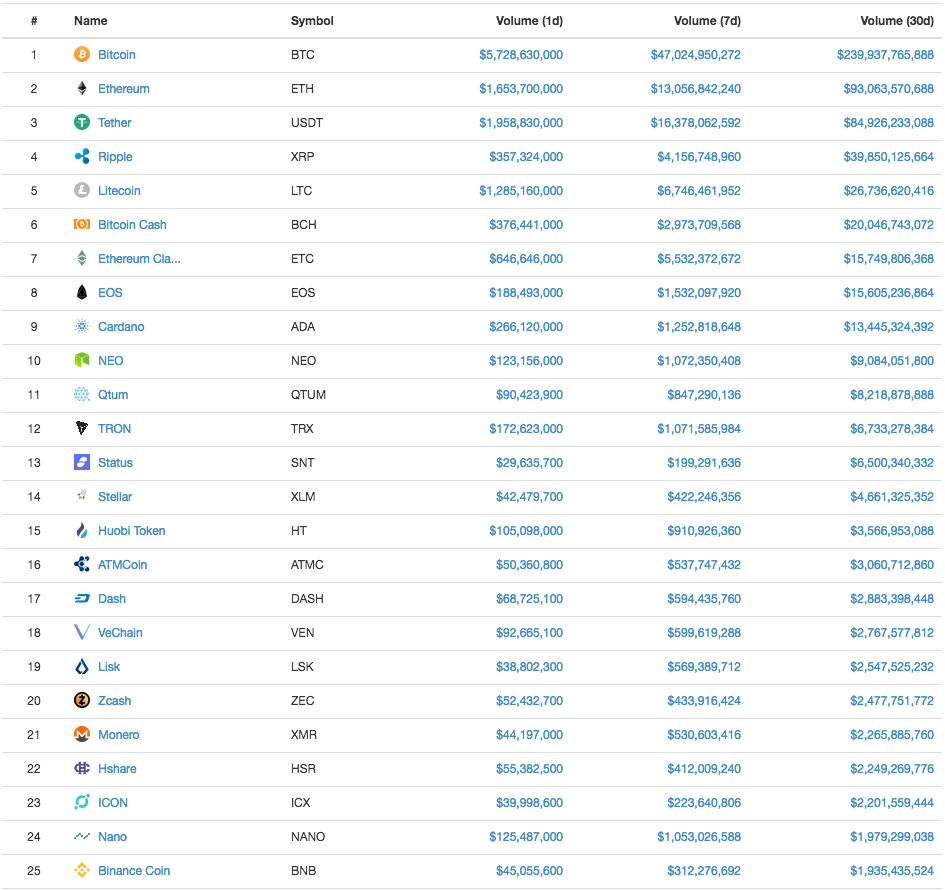
\includegraphics[width=0.6\textwidth]{figures/coinmarketcap}
    \caption[Snapshot Coinmarketcap] {
      Meest verhandelde cryptocurrencies in de maand februari zoals gepresenteerd op de website van Coinmarketcap.
    }
    \label{coinmarketcap}
  \end{center}
\end{wrapfigure}
Een van de overzichten is het maandelijkse handelsvolume zoals te zien in fig. \ref{coinmarketcap}. Deze lijst is gebruikt voor het selecteren van de initiële top 20 van cryptocurrencies. Door de architecturen achter de meest verhandelde cryptocurrencies te gebruiken wordt ervoor gezorgd dat er robuuste en volwassen implementaties bekeken worden.

\subsubsection{Hard forks}
Om te voorkomen dat er soortgelijke implementaties bekeken worden is ervoor gekozen om de hard forks niet mee te nemen in de initiële selectie. Een voorbeeld hiervan is Bitcoin Cash ten opzichte van Bitcoin. Alhoewel Bitcoin Cash een aantal veranderingen doorgemaakt heeft sinds de afsplitsing van het Bitcoin protocol, wordt het niet meegenomen omdat er in zekere mate overeenkomsten aanwezig zijn.

\section{Attributen}
Om een selectie te maken tussen de top 20 verhandelde cryptocurrencies is er gekeken naar attributen die nader beschreven zijn in onderstaand tabel.

\begin{centering}
  \begin{table}[ht]
    \label{selectie-attributen}
    \caption{Attributen opgesteld voor initiële selectie implementaties.}
    \makebox[\textwidth]{%
      \begin{tabular}{r|p{10cm}}
        \textbf{Identity Management} & Of de implementatie actief iets onderneemt dat te maken heeft met Identity Management, e.g.\ het vergroten van de privacy van de gebruiker. \\
        \hline
        \textbf{Whitepaper} & Of de implementatie een technische whitepaper beschikbaar heeft. \\
        \hline
        \textbf{Open-source} & Of er een referentie implementatie open-source beschikbaar is voor het bestuderen van de code. \\
        \hline
        \textbf{In circulatie sinds} & Een indicatie van de volwassenheid van de implementatie. \\ 
        \hline
        \textbf{DApps platform} & Of het gebruikt kan worden als development platform. Hierbij zal er een zekere mate van modulariteit nodig zijn in de broncode. \\ 
        \hline
        \textbf{Consensus} & Welk consensus algoritme gebruikt wordt. Dit is van invloed op de werking van het onderdeel Distributed Network. \\
      \end{tabular}
    }
  \end{table}
\end{centering}

Het doel van de attributen is een indicatie te krijgen over de hoeveelheid documentatie die een implementatie beschikbaar heeft. Dit is dan ook de doorslaggevende factor geweest bij het selecteren van vier implementaties die nader onderzocht zullen worden.

\newpage
\subsubsection{Totstandkoming}

Hieronder wordt kort beschreven hoe de inventarisatie van de attributen gedaan is.

\paragraph{Identity Management}
Om vast te stellen of een implementatie iets onderneemt in de vorm van Identity Management wordt er gebruik gemaakt van bestaande literatuur over de implementatie. Door middel van het scannend lezen van de beschikbare literatuur wordt er vastgesteld of er beschrijvingen zijn van de identiteit binnen de Blockchain implementatie en hoe dit tot stand is gekomen.

\paragraph{Whitepaper}
Bijna elke Blockchain implementatie heeft een website waarin de functionaliteiten gepresenteerd worden voor de mogelijke gebruiker. Om erachter te komen of er een whitepaper beschikbaar is, is een scan van de website voldoende.

\paragraph{Open-source}
Om na te gaan of een implementatie open-source is wordt er gezocht op Github en Bitbucket op de aanwezigheid van de organisatie en/of protocol naam.

\paragraph{In circulatie sinds}

Om de circulatiedatum te achterhalen is gebruik gemaakt van Wikipedia. Hierbij is een schatting van de datum waarop de Blockchain implementatie actief is geworden al voldoende.

\paragraph{DApps platform}

Om na te gaan of de implementatie de ontwikkeling van gedistribueerde applicaties ondersteund is er gezocht naar development tutorials op de websites van de Blockchain implementatie.

\paragraph{Consensus}

Het type consensus dat gebruikt wordt is tevens te achterhalen uit de besschikbare documentatie en wordt achterhaald door scannend te lezen.

\newpage
\section{Selectie}

Aan de hand van deze attributen is een lijst opgesteld, te zien in tabel \ref{bijlage_selectie_implementatie}, waarin de initiële selectie te vinden is met bijbehorende attributen van de implementatie. Over sommige implementaties zoals VeChain is weinig informatie gevonden waardoor ze direct afvallen. Aan de hand van deze attributen zijn de volgende protocollen geselecteerd.

\paragraph{Cardano} is een Blockchain protocol waarin onderzoek centraal staat. Het beweert dan ook het eerste blockchain platform te zijn die ontstaan is uit een filosofisch en onderzoek gedreven aanpak. De implementatie van het protocol is volledig open-source en er is een technische whitepaper beschikbaar. Daarnaast is er ook een platform om je eigen applicaties op het netwerk te creëren.

\paragraph{Monero} is een implementatie die beweert dat de gebruiker volledig ontraceerbaar is. Het is net zoals Cardano een volledige open-source implementatie en maakt gebruik van egalitair Proof of Work. Daarnaast heeft het protocol een technische whitepaper. 

\paragraph{Bitcoin} is het originele protocol waarin de Blockchain technologie gerealiseerd is. Door de grote hoeveelheid onderzoek die gedaan is naar Bitcoin is er een overvloed van informatie, waarin niet alleen informatie over Bitcoin gegeven wordt maar ook over het Blockchain domein. De implementatie van het protocol is wederom volledig open-source en er is een technische whitepaper beschikbaar.

\paragraph{EOS} is een relatief nieuw protocol die zojuist een test netwerk gelanceerd heeft. Ook deze implementatie is beschreven in een whitepaper, is volledig open-source en kan gebruikt worden als platform om applicaties op te ontwikkelen. Consensus binnen het protocol wordt bereikt door Delegated Proof of Stake.
